\section{Breakdown}

\subsection{Rationale}

	In aim 2, the design of the end effector and core tubing circuitry is addressed. In this portion of the project, the end effector will be engineered to house the TCP such that it is not exposed, can be replaced when necessary, does not limit its range of motion, and also allows for the installment of the camera and light. To achieve this, the four strands of TCP will be lined in parallel to the center tube, which contains the necessary assortment of circuit components. It should be noted that this task is not dependent on the completion on Aim 1, as the TCP wires can be replicated with past test wire or thick string, and can be given a maximum TCP diameter which satisfies the constraint that the full prototype fits in the endotracheal tube.

	The core tubing, which is extruded from the housing module and connects to the end effector via a specially designed clip, will likewise need to house the necessary wires which lead to the TCP, light and camera. This portion of the tubing will be relatively simple in configuration, with the primary limiting factor being the diameter of the tube.

	\begin{figure}[ht]
		\centering
		\includegraphics[scale=0.95]{prototype_assembly}
		\caption{Prototype Assembly Developed in 2021-2022 Academic Year by OSU Capstone Team}
		\label{fig:prototype_assembly}
	\end{figure}
	
	Figure \ref{fig:prototype_assembly} shows the prototype designed and assembled by the aforementioned OSU capstone team. This prototype was specifically designed with the intent to prove functionality, and thus many quality-of-life features were not included. The most noticeable example of this being the exposed wiring at the prototype end effector, and the imprecise method of connection to the TCP ground wire. As this is the project being expanded upon, the previous prototype will be used as a reference for the general configuration of the tubing but will be largely redesigned.

\subsection{Approach}

	\subsubsection{Timeline}
	
		The timeline for the design and creation of the continuum snake will likely be more sequatial than in Aim 1. Each of the components; the end effector, the core tubing and the connection between them, will be broken into itemized sections. More specifically, the end effector design segment, will most likely require close to $40\%$ of the total project time. That is, for a year-long project, the end effector would be designated approximately $5[months]$. This time is primarily split between researching airway-compatible flexible materials, and designing the internal layout for the TCP, camera and light configuration. It should be noted here that the circuit which controls the current to the inividual TCP wires (without the camera/light) was created during the OSU capstone project, and will likely not be changed dramatically here. This circuit can be seen in Figure \ref{fig:tcp_circuit}. The steps for this task are highlighted in lines 23-29 of Figure \ref{fig:full_timeline}.
		
		In the next segment, about $25\%$ of project time will be appropriated to the design and creation of the core tubing (about $3[months]$ for a year-long project). This portion of the project is fundamentally simpler when compared to the first task, and is not seen as a large risk to project time. That said, the connection mechanism which allows for the smooth replacement of the end effector in the event of a breakage will be extremely important since the end effector is dependent on the wire connections and must be properly secured (shown in lines 30-35 of the Full Timeline).
		
		The design of the connection mechanism will occur after both the end effector and core tubing are completed, and is appointed $25\%$ of the total project time ($3[months]$ for a year-long project). This is because of the important of this feature to the fast application necessary in the emergency environment. The remaining $10\%$ of the project will be left open in the event that one or more of the sections requires slightly more time to be completed to the necessary standard.
		
		The completed timeline, as well as those constructed for Aim 1 and 3, is shown in Figure \ref{fig:full_timeline}.
	
	\subsubsection{Tubing/Circuitry Techniques}

		The end effector will be constructed with the intent of a two-layer configuration. The center will be comprised of the ground wire and the camera, similar to the prototype made during the OSU capstone project with an insulating tube surrounding the components (layer 1). Next, the TCP will be connected in parallel around the center shaft and connected to the common ground wire. Each string will also be connected to an individual active wire which is used to control the current supplied to the TCP from the main controller. The TCP will then be surrounded by another layer of insulated tubing (layer 2). It is also possible that a third intermediate layer will be introduced to insulate the individual TCP string from one another, this will hopefully be avoidable though as it would unnecessarily increase the diameter of the assembled system. This portion of the device will only span one to two inches in length. Note that the controller need not be completed for testing, in initial scenarios, a simple user-defined analog signal can be used to test motion.
		
		\begin{figure}[ht]
			\centering
			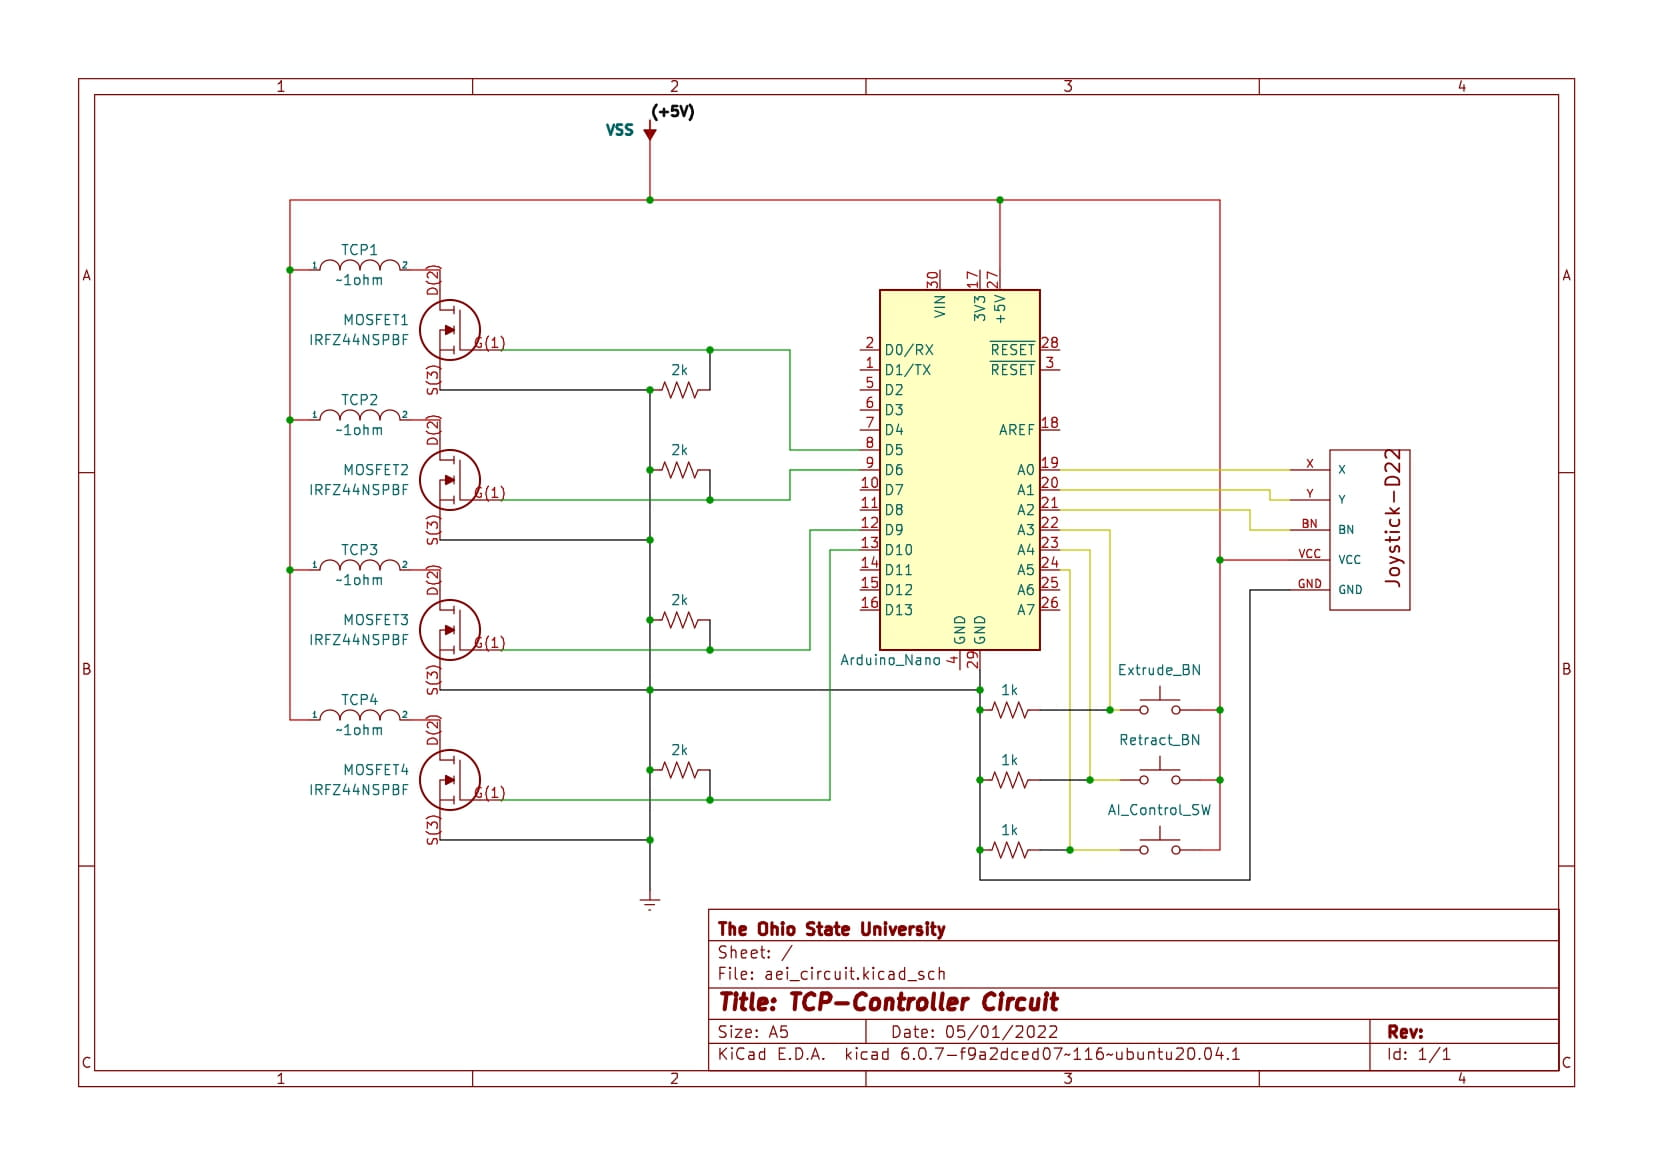
\includegraphics[scale=0.27, trim={2.75cm 2.75cm 2.75cm 2.75cm}, clip=true]{tcp_circuit}
			\caption{TCP Circuit Created in OSU Capstone Project}
			\label{fig:tcp_circuit}
		\end{figure}
		
		The TCP circuit is made up of three primary components; the four TCP strands and their designated MOSFET transistor which controls the variable current magnitude, the joystick which acts as a vehicle for manual operation of the end effector, and three buttons which control the extrusion, retraction, and AI features. The bulk of these items are housed in the control module (shown in Figure \ref{fig:prototype_assembly}), leaving the TCP as the only remaining item which must be included in the end effector.

		The core tubing will be considerably simpler to assemble and can be stylized to a single airway-compatible tube housing the necessary wires which will each be individually insulated. This is similar to every day USB pin-out wiring and other related cords. Because of its simplicity, the core tubing is not likely to break or have technical issues after being assembled. For this reason, the end effector and core tubing will be design separately and connected together via a locking mechanism. This way, if the end effector malfunctions, it can be replaced relatively easily, and without affecting the rest of the assembly. It may also be necessary to incorporate a aesthetic center-line down both components such that they can be attached to one another in a consistent configuration.
	
	\subsubsection{Experimental Process}
	
		The experimental process practiced here will primarily be focused on patient compatibility, end effector flexibility, and dimension fitting. Since the prototype is obselete if the end effector does not fit within the confines of the intubation tube, this specification will be prioritized. TCP string is known for its high degree of flexbility, one reason why it is ideal for working in such a tight environment \cite{haines_new_2016}. That said, the inner components will most likely have to be optimized such that the dimension tests can be fulfilled reliably.
		
		Flexibility tests will occur for the two main components seperately, as well as for the final assembly, and are represneted by schedule items 28, 34 and 43 in Figure \ref{fig:full_timeline}. The end effector must be able to freely stretch in all directions in the full assembly while the core tubing should be slightly more rigid, allowing it to be extruded from the control module reliably. Pass/fail parameters for these tests will be defined more thoroughly before the project start.
		
		The final test is the compatibility test and will likely be non-pervasive, which is why it is not referenced directly on the project timeline. This test is to ensure the materials being utilized are compatible with the human airway anatomy, and do not pose any form of danger to the patient. To account for this during the design process, only pre-approved anatomy-compatible materials will be considered for the composition of the end effector, core tubing and connector segments. For this reason, the testing of the materials is not given scheduling time.

\subsection{Risks and Alternatives}

	The largest risk being addressed in this portion of development is the hard constraint for the diameter of the tubing. The most complex portion of the tubing, the end effector, must fit within the confines of commonly used intubating tubes. For development purposes, the constraint can be relaxed to the smallest adult-specific tube available ($8[mm]$ diameter). This will likely be more than enough room for the current configuration since the OSU capstone project final design was very close to fitting comfortably, despite having many imperfections in the design of the end effector.
	
	It should also be noted that the circuit diagram referenced in Figure \ref{fig:tcp_circuit} does not include the end effector light or camera, meaning it will have to be incorporated during the project planning period. The system will likely resemble the current flexibile intubation scope camera/light system, although more research is required before making the final adjustments to the circuit.